\section{Three-Dimensional Coordinate Systems}
  An ordered pair $(a,\ b)$ of real numbers is used to represent a point in a plane, which is two-dimensional. To locate a point in space, which is three-dimensional, we use an ordered triple $(a,\ b,\ c)$ of real numbers.
  \begin{center}
    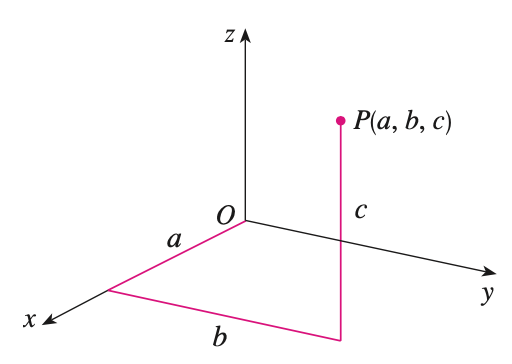
\includegraphics[width=0.6\textwidth]{coordinate.png}
  \end{center}
  To represent points in space we draw three perpendicular lines, called the \textbf{coordinate axes} and labeled the $x$-axis, $y$-axis, and $z$-axis, through a fixed point $O$ (the origin). The three coordinate axes determine the three \textbf{coordinate planes}: the $xy$-plane contains the $x$- and $y$-axes; the $yz$-plane contains the $y$- and $z$-axes; the $xz$-plane contains the $x$- and $z$-axes. The three coordinate planes divided space into eight parts called \textbf{octants}. The \textbf{first octant} is the side we typically see and represents the positive axes.\par
  If $P$ is any point in space, let $a$ be the $x$-coordinate, let $b$ be the $y$-coordinate, and let $c$ be the $z$-coordinate. We represent point $P$ by the ordered triple $(a,\ b,\ c)$. If we drop a perpendicular from $P$ to the $xy$-plane, we get a point $Q$ with coordinates $(a,\ b,\ 0)$ called the \textbf{projection} of $P$ on the $xy$-plane. Similarly, $R(0,\ b,\ c)$ is the projection of $P$ on the $yz$-plane and $S(a,\ 0,\ c)$ is the projection of $P$ on the $xz$-plane.\par
  The Cartesian product $\mathbb{R} \times \mathbb{R} \times \mathbb{R} = \{(x,y,z)|x,y,z \in \mathbb{R}\}$ is the set of all ordered triples of real numbers and is denoted by $\mathbb{R}^3$. This is called a \textbf{three-dimensional rectangular coordinate system}.\par
  In two-dimensional analytic geomemtry, the graph of an equation involving $x$ and $y$ is a \textbf{curve} in $\mathbb{R}^2$. In three-dimensional analytic geomemtry, an equation in $x$, $y$, and z is a \textbf{surface} in $\mathbb{R}^3$.
  \\~\\
  The formula for distance between two points in a plane is easily extended to a formula for three dimensions.
  \begin{definition}[\textbf{Distance Formula in Three Dimensions}]
    The distance $|P_1 P_2|$ between the points $P_1 (x_1,y_1,z_1)$ and $P_2 (x_2,y_2,z_2)$ is
    $$|P_1 P_2| - \sqrt{(x_2 - x_1)^2 + (y_2 - y_1)^2 + (z_2 - z_1)^2}$$
  \end{definition}
  \begin{proof}\let\qed\relax
    Construct a rectangular box where $P_1$ and $P_2$ are opposite vertices and the sides of the box is parallel to the coordinate planes.
    \begin{center}
      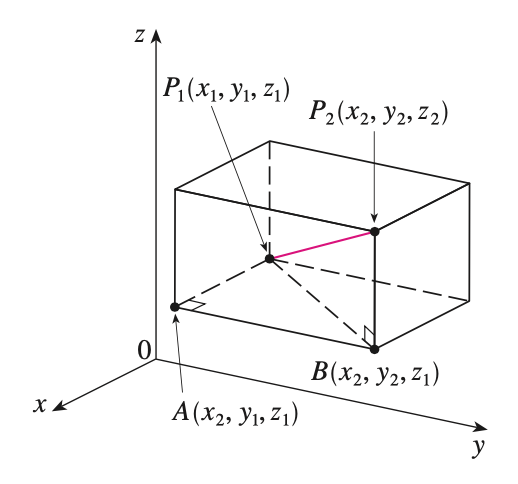
\includegraphics[width=0.4\textwidth]{distance.png}
    \end{center}
    If $A(x_2,y_1,z_1)$ and $B(x_2,y_2,z_1)$ are the vertices of the box indicated in the figure, then
    $$|P_1 A| = |x_2 - x_1| \qquad |AB| = |y_2 - y_1| \qquad |BP_2| = |z_2 - z_1|$$
    Because triangles $P_1 BP_2$ and $P_1 AB$ are both right triangles, two applications of the Pythagorean Theorem give
    \begin{align*}
      |P_1 P_2|^2 &= |P_1 B|^2 + |BP_2|^2 \\
      |P_1 B|^2 &= |P_1 A|^2 + |AB|^2
    \end{align*}
    Combine these equations through substitution to get
    \begin{align*}
      |P_1 P_2|^2 &= |P_1 A|^2 + |AB|^2 + |BP_2|^2 \\
      &= |x_2 - x_1|^2 + |y_2 - y_1|^2 + |z_2 - z_1|^2 \\
      &= (x_2 - x_1)^2 + (y_2 - y_1)^2 + (z_2 - z_1)^2 \\
      &= \sqrt{(x_2 - x_1)^2 + (y_2 - y_1)^2 + (z_2 - z_1)^2}
    \end{align*}
  \end{proof}
  \begin{example}
    The distance from point $P(2,-1,7)$ to the point $Q(1,-3,5)$ is
    $$ |PQ| = \sqrt{(1 - 2)^2 + (-3 - 1)^2 + (5 - 7)^2} = \sqrt{1+4+4} = 3$$
  \end{example}
  Just as the two-dimensional distance formula can be used to define the equation of a circle, the three-dimensional distance formula can be used to define the equaition of a sphere.
  \begin{definition}[\textbf{Equation of a Sphere}]
    An equation of a sphere with center $C(h,k,l)$ and radius $r$ is
    $$(x-h)^2 + (y-k)^2 + (z-l)^2 = r^2$$
    In particular, if the center is the origin $O$, then an equation of the sphere is
    $$x^2 + y^2 + z^2 = r^2$$
  \end{definition}
  \begin{proof}\let\qed\relax
    By definition, a sphere is the set of all points $P(x,y,z)$ whos distance from center $C(h,k,l)$ is radius $r$. Thus, $P$ is on the sphere if and only if $|PC|=r$. Squaring both sides, we have $|PC|^2=r^2$, or
    $$(x-h)^2 + (y-k)^2 + (z-l)^2 = r^2$$
  \end{proof}
  \begin{example}
    Show that $x^2 + y^2 + z^2 + 4x - 6y + 2z + 6 = 0$ is the equation of a sphere, and find its center and radius.
  \end{example}
  \begin{solution}
    We can rewrite the given equation in the form of an equation of a sphere by completing the square:
    \begin{align*}
      (x^2 + 4x + 4) + (y^2 - 6y + 9) (z^2 + 2z + 1) &= -6 + 4 + 9 + 1 \\
      (x+2)^2 + (y-3)^2 + (z+1)^2 &= 8
    \end{align*}
    Comparing this equation with the standard form, we see that it is the equation of a sphere with center $(-2,3,-1)$ and radius $\sqrt{8} = 2\sqrt{2}$.
  \end{solution}
  \begin{example}
    What region in $\mathbb{R}^3$ is represented by $ 1 \leq x^2 + y^2 + z^2 \leq 4,\; z \leq 0$?
  \end{example}
  \begin{solution}
    Rewrite the inequality as $1 \leq \sqrt{x^2 + y^2 + z^2} \leq 2$, which represents the points whose distance from the origin  is at least 1 and at most 2. Since $z \leq 0$, the points lie on or below the $xy$-plane. The inequalities represent the lower hemisphere between the radii 1 and 2.
  \end{solution}
